\documentclass{beamer}
\usetheme{metropolis}

\usepackage[spanish]{babel}
\usepackage[utf8]{inputenc}
\usepackage{graphicx}
\usepackage{tikz}
\usepackage{xcolor}
\usepackage{amsmath}
\usepackage{listings}

% Definición de colores personalizados
\definecolor{primary}{RGB}{46, 204, 113}
\definecolor{secondary}{RGB}{52, 152, 219}
\definecolor{accent}{RGB}{231, 76, 60}
\definecolor{background}{RGB}{236, 240, 241}
\definecolor{gradient1}{RGB}{255, 107, 107}
\definecolor{gradient2}{RGB}{255, 159, 67}

% Configuración del tema
\setbeamercolor{normal text}{fg=black,bg=background}
\setbeamercolor{structure}{fg=primary}
\setbeamercolor{alerted text}{fg=accent}

\definecolor{lightgray}{rgb}{0.95,0.95,0.95}
\definecolor{darkgreen}{rgb}{0,0.5,0}
\definecolor{darkblue}{rgb}{0,0,0.5}

\lstset{
  backgroundcolor=\color{lightgray},
  basicstyle=\tiny\ttfamily,
  keywordstyle=\color{darkblue}\bfseries,
  commentstyle=\color{darkgreen},
  stringstyle=\color{red},
  numbers=left,
  numberstyle=\tiny\color{gray},
  stepnumber=1,
  numbersep=5pt,
  showspaces=false,
  showstringspaces=false,
  showtabs=false,
  frame=single,
  tabsize=2,
  language=Python,
  breaklines=true,
  breakatwhitespace=true
}

\title{\Huge\textbf{Validación de Modelos}}
\author{Analítica de Datos, Universidad de San Andrés}
\date{}

\begin{document}

\begin{frame}
    \titlepage
    \begin{tikzpicture}[remember picture,overlay]
        \node[anchor=south west,inner sep=30pt] at (current page.south west) {
            
\includegraphics[height=1cm]{../misc/UdeSA.png}
        };
    \end{tikzpicture}
\end{frame}

\begin{frame}{Tipos de Problemas en Machine Learning}
    \begin{columns}
        \begin{column}{0.5\textwidth}
            \textbf{Regresión}
            \begin{itemize}
                \item Predecir números
                \item Ejemplos:
                \begin{itemize}
                    \item Precio de casas
                    \item Temperatura
                    \item Salario
                \end{itemize}
            \end{itemize}
        \end{column}
        \begin{column}{0.5\textwidth}
            \textbf{Clasificación}
            \begin{itemize}
                \item Predecir categorías o clases
                \item Ejemplos:
                \begin{itemize}
                    \item Spam/No spam
                    \item Enfermedad/Sano
                    \item Compra/No compra
                \end{itemize}
            \end{itemize}
        \end{column}
    \end{columns}
    
    \vspace{1em}
    \begin{center}
        \Large \textbf{¡Cada tipo requiere métricas de validación específicas!}
    \end{center}
\end{frame}

\begin{frame}{Validación para Regresión}
    \begin{center}
        \Large En regresión medimos qué tan \textbf{cerca} están nuestras predicciones de los valores reales
    \end{center}
    
    \vspace{1em}
    
    \begin{itemize}
        \onslide<2->{\item \textbf{MSE}: Mean Squared Error}
        \onslide<3->{\item \textbf{RMSE}: Root Mean Squared Error}
        \onslide<4->{\item \textbf{MAE}: Mean Absolute Error}
        \onslide<5->{\item \textbf{R²}: R-squared}
        \onslide<6->{\item \textbf{MAPE}: Mean Absolute Percentage Error}
    \end{itemize}
\end{frame}

\begin{frame}{MSE - Mean Squared Error}
    \begin{center}
        \Large MSE = $\frac{1}{n} \sum_{i=1}^{n} {(y_i - \hat{y}_i)}^2$
    \end{center}
    
    \begin{itemize}
        \item Penaliza más los errores grandes
        \item Sensible a valores atípicos
        \item Unidades al cuadrado de la variable objetivo
    \end{itemize}
\end{frame}

\begin{frame}{RMSE - Root Mean Squared Error}
    \begin{center}
        \Large RMSE = $\sqrt{\text{MSE}} = \sqrt{\frac{1}{n} \sum_{i=1}^{n} {(y_i - \hat{y}_i)}^2}$
    \end{center}
    
    \begin{itemize}
        \item Mismas unidades que la variable objetivo
        \item Más fácil de interpretar que MSE
        \item Mantiene la penalización por errores grandes
    \end{itemize}
\end{frame}

\begin{frame}{MAE - Mean Absolute Error}
    \begin{center}
        \Large MAE = $\frac{1}{n} \sum_{i=1}^{n} |y_i - \hat{y}_i|$
    \end{center}
    
    \begin{itemize}
        \item Menos sensible a valores atípicos
        \item Mismas unidades que la variable objetivo
        \item Trata todos los errores por igual
    \end{itemize}
\end{frame}

\begin{frame}{R² - R-squared}
    \begin{center}
        \Large R² = $1 - \frac{\sum_{i=1}^{n} {(y_i - \hat{y}_i)}^2}{\sum_{i=1}^{n} {(y_i - \bar{y})}^2}$
    \end{center}
    
    \begin{itemize}
        \item R² = 1: Modelo perfecto
        \item R² = 0: Modelo no mejor que la media
        \item R² $<$ 0: Modelo peor que la media
    \end{itemize}
\end{frame}

\begin{frame}{MAPE - Mean Absolute Percentage Error}
    \begin{center}
        \Large MAPE = $\frac{100\%}{n} \sum_{i=1}^{n} \left|\frac{y_i - \hat{y}_i}{y_i}\right|$
    \end{center}
    
    \begin{itemize}
        \item Error expresado como porcentaje
        \item Fácil de interpretar
        \onslide<2->{\item \textbf{Problema:} División por cero cuando $y_i = 0$}. Podemos solucionar reemplazando los que sean cero por un valor tipo 0.0000001, filtrar ceros, entre otras cosas.
    \end{itemize}
\end{frame}

\begin{frame}{Ejemplo Práctico de Regresión}
    \begin{center}
        \begin{tabular}{|c|c|c|}
        \hline
        \textbf{Casa} & \textbf{Precio Real} & \textbf{Precio Predicho} \\
        \hline
        1 & 30 & 28 \\
        2 & 45 & 47 \\
        3 & 20 & 19 \\
        4 & 60 & 62 \\
        5 & 35 & 33 \\
        \hline
        \end{tabular}
    \end{center}
    
    \vspace{1em}
    
    \begin{columns}
        \begin{column}{0.5\textwidth}
            \begin{itemize}
                \onslide<2->{\item MSE} \onslide<3->{= 18}
                \onslide<4->{\item RMSE} \onslide<5->{= 4.24}
                \onslide<6->{\item MAE} \onslide<7->{= 3.6}
            \end{itemize}
        \end{column}
        \begin{column}{0.5\textwidth}
            \begin{itemize}
                \onslide<8->{\item R²} \onslide<9->{= 0.95}
                \onslide<10->{\item MAPE} \onslide<11->{= 4.95\%}
            \end{itemize}
        \end{column}
    \end{columns}
\end{frame}

\begin{frame}{Validación para Clasificación}
    \begin{center}
        \Large En clasificación medimos la precisión de las predicciones categóricas
    \end{center}
    
    \vspace{1em}
    
    \begin{itemize}
        \item Matriz de Confusión
        \item Métricas básicas (Accuracy, Precision, Recall, etc.)
        \item Métricas avanzadas (ROC, AUC, PR)
        \item Casos de uso específicos
    \end{itemize}
\end{frame}

\begin{frame}{Matriz de Confusión Binaria}
    \begin{center}
    \begin{tikzpicture}[scale=0.8]
    \draw (0,0) rectangle (4,4);
    \draw (0,2) -- (4,2);
    \draw (2,0) -- (2,4);
    
    \node[above] at (2,4) {\textbf{Real}};
    \node[left] at (0,2) {\textbf{Predicho}};
    
    \fill[green!30] (0,2) rectangle (2,4);
    \fill[red!30] (2,0) rectangle (4,2);
    \fill[blue!30] (0,0) rectangle (2,2);
    \fill[yellow!30] (2,2) rectangle (4,4);
    
    \node at (1,3) {VP};
    \node at (3,3) {FP};
    \node at (1,1) {FN};
    \node at (3,1) {VN};
    \end{tikzpicture}
    \hspace{0.5cm}
    \begin{tikzpicture}[scale=0.8]
    \draw (0,0) rectangle (4,4);
    \draw (0,2) -- (4,2);
    \draw (2,0) -- (2,4);
    
    \node[above] at (2,4) {\textbf{Predicho}};
    \node[left] at (0,2) {\textbf{Real}};
    
    \fill[green!30] (0,2) rectangle (2,4);
    \fill[red!30] (2,0) rectangle (4,2);
    \fill[yellow!30] (0,0) rectangle (2,2);
    \fill[blue!30] (2,2) rectangle (4,4);
    
    \node at (1,3) {VP};
    \node at (3,3) {FN};
    \node at (1,1) {FP};
    \node at (3,1) {VN};
    \end{tikzpicture}
    \end{center}
    
    \begin{itemize}
        \item VP: Verdaderos Positivos
        \item VN: Verdaderos Negativos
        \item FP: Falsos Positivos
        \item FN: Falsos Negativos
    \end{itemize}
\end{frame}

\begin{frame}{Matriz de Confusión Multiclase}
    \begin{center}
    \begin{tikzpicture}[scale=0.7]
    \node[above] at (3,7) {\textbf{R}};
    \node[left] at (-1,3) {\textbf{P}};
    
    \draw (0,0) rectangle (6,6);
    \draw (0,2) -- (6,2);
    \draw (0,4) -- (6,4);
    \draw (2,0) -- (2,6);
    \draw (4,0) -- (4,6);
    
    \fill[green!30] (0,4) rectangle (2,6);
    \fill[green!30] (2,2) rectangle (4,4);
    \fill[green!30] (4,0) rectangle (6,2);
    
    \node at (1,5) {85};
    \node at (3,5) {10};
    \node at (5,5) {5};
    \node at (1,3) {8};
    \node at (3,3) {82};
    \node at (5,3) {10};
    \node at (1,1) {7};
    \node at (3,1) {12};
    \node at (5,1) {81};
    
    \node at (-0.5,5) {L};
    \node at (-0.5,3) {N};
    \node at (-0.5,1) {S};
    
    \node at (1,6.5) {L};
    \node at (3,6.5) {N};
    \node at (5,6.5) {S};
    \end{tikzpicture}
    \end{center}
    
    \begin{itemize}
        \item L: Lluvia
        \item N: Nublado
        \item S: Soleado
    \end{itemize}
\end{frame}

\begin{frame}{Accuracy (Exactitud)}
    \begin{center}
    \Large Accuracy = $\frac{\colorbox{green!30}{VP} + \colorbox{red!30}{VN}}{\colorbox{green!30}{VP} + \colorbox{red!30}{VN} + \colorbox{yellow!30}{FP} + \colorbox{blue!30}{FN}}$
    \end{center}
    Es el porcentaje total de predicciones correctas que hace nuestro modelo.
\end{frame}

\begin{frame}{Precision (Precisión)}
    \begin{center}
    \Large Precision = $\frac{\colorbox{green!30}{VP}}{\colorbox{green!30}{VP} + \colorbox{yellow!30}{FP}}$
    \end{center}
    Es qué tan confiables son nuestras predicciones positivas.
\end{frame}

\begin{frame}{Specificity (Especificidad) / True Negative Rate (TNR)}
    \begin{center}
    \Large Specificity = $\frac{\colorbox{red!30}{VN}}{\colorbox{red!30}{VN} + \colorbox{yellow!30}{FP}}$
    \end{center}
    Es qué tan bien identificamos los casos negativos correctamente.
\end{frame}

\begin{frame}{Recall (Sensibilidad) / True Positive Rate (TPR)}
    \begin{center}
    \Large Recall (TPR) = $\frac{\colorbox{green!30}{VP}}{\colorbox{green!30}{VP} + \colorbox{blue!30}{FN}}$
    \end{center}
    Es qué tan bien detectamos todos los casos positivos que existen.
\end{frame}

\begin{frame}{Fall-out / False Positive Rate (FPR)}
    \begin{center}
    \Large Fall-out (FPR) = $\frac{\colorbox{yellow!30}{FP}}{\colorbox{yellow!30}{FP} + \colorbox{red!30}{VN}}$
    \end{center}
    Es qué tan seguido nos equivocamos prediciendo casos positivos.
\end{frame}

\begin{frame}{Miss Rate / False Negative Rate (FNR)}
    \begin{center}
    \Large Miss Rate (FNR) = $\frac{\colorbox{blue!30}{FN}}{\colorbox{blue!30}{FN} + \colorbox{green!30}{VP}}$
    \end{center}
    Es qué tan seguido nos perdemos casos positivos que deberíamos haber detectado.
\end{frame}

\begin{frame}{F1-Score}
    \begin{center}
    \Large F1-Score = $2 \times \frac{Precision \times Recall}{Precision + Recall}$
    \end{center}
    Es un balance entre la precisión y el recall, útil cuando las clases están desbalanceadas.
\end{frame}

\begin{frame}{False Discovery Rate (FDR)}
    \begin{center}
    \Large FDR = $\frac{\colorbox{yellow!30}{FP}}{\colorbox{yellow!30}{FP} + \colorbox{green!30}{VP}}$
    \end{center}
    Es qué tan seguido nos equivocamos cuando hacemos predicciones positivas.
\end{frame}

\begin{frame}{False Omission Rate (FOR)}
    \begin{center}
    \Large FOR = $\frac{\colorbox{blue!30}{FN}}{\colorbox{blue!30}{FN} + \colorbox{red!30}{VN}}$
    \end{center}
    Es qué tan seguido nos equivocamos cuando hacemos predicciones negativas.
\end{frame}

\begin{frame}{Negative Predictive Value (NPV)}
    \begin{center}
    \Large NPV = $\frac{\colorbox{red!30}{VN}}{\colorbox{red!30}{VN} + \colorbox{blue!30}{FN}}$
    \end{center}
    Es qué tan confiables son nuestras predicciones negativas.
\end{frame}

\begin{frame}{Curva ROC}
    \begin{center}
    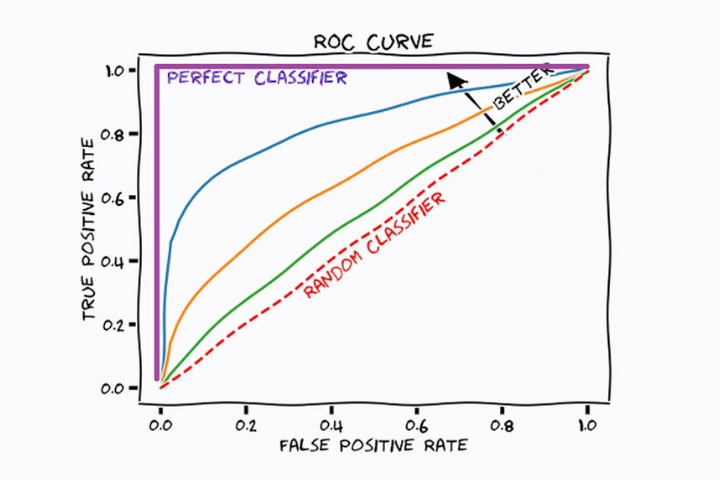
\includegraphics[width=0.7\textwidth]{img/curva-roc.png}
    \end{center}

    La curva ROC muestra la relación entre TPR y FPR para diferentes umbrales. El área bajo la curva (AUC) indica el rendimiento del modelo.
\end{frame}

\begin{frame}{¿Cómo entender la curva ROC?}

    Para cada punto de umbral existe una tasa de falsos positivos y una tasa de verdaderos positivos. Las coordenadas que trazamos son (FPR, TPR) en el eje X e Y respectivamente. Recordamos que:

    \vspace{1em}

    \begin{center}
    Fall-out (FPR) = $\frac{\colorbox{yellow!30}{FP}}{\colorbox{yellow!30}{FP} + \colorbox{red!30}{VN}}$

    Recall (TPR) = $\frac{\colorbox{green!30}{VP}}{\colorbox{green!30}{VP} + \colorbox{blue!30}{FN}}$
    \end{center}
\end{frame}

\begin{frame}{Umbral 0 - Clasificar todo como positivo (1/2)}
    En el caso de un umbral 0, todo esta siendo calificado como positivo porque esta a la derecha del umbral, entonces:

    \begin{center}
    \begin{tikzpicture}
    \draw (0,0) rectangle (4,4);
    \draw (0,2) -- (4,2);
    \draw (2,0) -- (2,4);
    
    \node[above] at (2,4) {\textbf{R}};  
    \node[left] at (0,2) {\textbf{P}};
    
    \fill[green!30] (0,2) rectangle (2,4);
    \fill[red!30] (2,0) rectangle (4,2);
    \fill[blue!30] (0,0) rectangle (2,2);
    \fill[yellow!30] (2,2) rectangle (4,4);
    
    \node at (1,3) {$\alpha$ (VP)};
    \node at (3,3) {$\beta$ (FP)};
    \node at (1,1) {0 (FN)};
    \node at (3,1) {0 (VN)};
    
    \end{tikzpicture}
    \end{center}
\end{frame}

\begin{frame}{Umbral 0 - Clasificar todo como positivo (2/2)}
    \begin{center}
    Fall-out (FPR) = $\frac{\colorbox{yellow!30}{FP}}{\colorbox{yellow!30}{FP} + \colorbox{red!30}{VN}} = \frac{\colorbox{yellow!30}{$\beta$}}{\colorbox{yellow!30}{$\beta$} + \colorbox{red!30}{0}} = 1$

    Recall (TPR) = $\frac{\colorbox{green!30}{VP}}{\colorbox{green!30}{VP} + \colorbox{blue!30}{FN}} = \frac{\colorbox{green!30}{$\alpha$}}{\colorbox{green!30}{$\alpha$} + \colorbox{blue!30}{0}} = 1$
    \end{center}
\end{frame}

\begin{frame}{Umbral 1 - Clasificar todo como negativo (1/2)}
    En el caso de un umbral 1, todo esta siendo calificado como negativo porque esta a la izquierda del umbral, entonces:

    \begin{center}
    \begin{tikzpicture}
    \draw (0,0) rectangle (4,4);
    \draw (0,2) -- (4,2);
    \draw (2,0) -- (2,4);
    
    \node[above] at (2,4) {\textbf{R}};  
    \node[left] at (0,2) {\textbf{P}};
    
    \fill[green!30] (0,2) rectangle (2,4);
    \fill[red!30] (2,0) rectangle (4,2);
    \fill[blue!30] (0,0) rectangle (2,2);
    \fill[yellow!30] (2,2) rectangle (4,4);
    
    \node at (1,3) {0 (VP)};
    \node at (3,3) {0 (FP)};
    \node at (1,1) {$\alpha$ (FN)};
    \node at (3,1) {$\beta$ (VN)};
    
    \end{tikzpicture}
    \end{center}
\end{frame}

\begin{frame}{Umbral 1 - Clasificar todo como negativo (2/2)}
    \begin{center}
    Fall-out (FPR) = $\frac{\colorbox{yellow!30}{FP}}{\colorbox{yellow!30}{FP} + \colorbox{red!30}{VN}} = \frac{\colorbox{yellow!30}{0}}{\colorbox{yellow!30}{0} + \colorbox{red!30}{$\beta$}} = 0$

    Recall (TPR) = $\frac{\colorbox{green!30}{VP}}{\colorbox{green!30}{VP} + \colorbox{blue!30}{FN}} = \frac{\colorbox{green!30}{0}}{\colorbox{green!30}{0} + \colorbox{blue!30}{$\alpha$}} = 0$
    \end{center}
\end{frame}

\begin{frame}{Curva PR}
La curva PR (Precision-Recall) es similar a la ROC pero con métricas diferentes:

\begin{itemize}
    \item Eje X: Precisión
    \item Eje Y: Recall
\end{itemize}

\vspace{0.5em}

Para cada umbral U:
\begin{itemize}
    \item Calculamos precisión = $\frac{\colorbox{green!30}{VP}}{\colorbox{green!30}{VP} + \colorbox{yellow!30}{FP}}$
    \item Calculamos recall = $\frac{\colorbox{green!30}{VP}}{\colorbox{green!30}{VP} + \colorbox{blue!30}{FN}}$
\end{itemize}
\end{frame}

\begin{frame}{¿Cuándo usar la curva PR?}
La curva PR es especialmente útil cuando:
\begin{itemize}
    \item Tenemos clases desbalanceadas
    \item Nos interesa más la precisión que los falsos positivos
    \item El costo de los falsos negativos es alto
\end{itemize}
\end{frame}


\begin{frame}{Casos de Uso}
    \textbf{Salud}
    \begin{itemize}
        \item Priorizar recall sobre precisión
        \item Usar curvas PR
        \item No usar accuracy como métrica principal
    \end{itemize}
    
    \vspace{0.5em}
    
    \textbf{Justicia}
    \begin{itemize}
        \item Usar curvas ROC
        \item Considerar impacto social
        \item Evaluar transparencia
    \end{itemize}
\end{frame}

\begin{frame}{Ejemplo Práctico}
    \begin{center}
    \begin{tikzpicture}[scale=0.8]
    \draw (0,0) rectangle (4,4);
    \draw (0,2) -- (4,2);
    \draw (2,0) -- (2,4);
    
    \node[above] at (2,4) {\textbf{R}};
    \node[left] at (0,2) {\textbf{P}};
    
    \fill[green!30] (0,2) rectangle (2,4);
    \fill[red!30] (2,0) rectangle (4,2);
    \fill[blue!30] (0,0) rectangle (2,2);
    \fill[yellow!30] (2,2) rectangle (4,4);
    
    \node at (1,3) {80};
    \node at (3,3) {20};
    \node at (1,1) {10};
    \node at (3,1) {90};
    \end{tikzpicture}
    \end{center}
    
    {\small
    \begin{columns}
        \begin{column}{0.52\textwidth}
             \begin{itemize}
                 \onslide<2->{\item Accuracy} \onslide<3->{= $\frac{80 + 90}{200}$} \onslide<4->{= 0.85}
                 \onslide<5->{\item Precision} \onslide<6->{= $\frac{80}{90}$} \onslide<7->{= 0.89}
                 \onslide<8->{\item Specificity (TNR)} \onslide<9->{= $\frac{90}{100}$} \onslide<10->{= 0.90}
                 \onslide<11->{\item Recall (TPR)} \onslide<12->{= $\frac{80}{100}$} \onslide<13->{= 0.80}
                 \onslide<14->{\item Fall-out (FPR)} \onslide<15->{= $\frac{10}{100}$} \onslide<16->{= 0.10}
             \end{itemize}
        \end{column}
        \begin{column}{0.50\textwidth}
            \begin{itemize}
                \onslide<17->{\item Miss Rate (FNR)} \onslide<18->{= $\frac{20}{100}$} \onslide<19->{= 0.20}
                \onslide<20->{\item F1} \onslide<21->{= $2 \times \frac{0.89 \times 0.80}{0.89 + 0.80}$} \onslide<22->{= 0.84}
                \onslide<23->{\item FDR} \onslide<24->{= $\frac{10}{90}$} \onslide<25->{= 0.11}
                \onslide<26->{\item FOR} \onslide<27->{= $\frac{20}{110}$} \onslide<28->{= 0.18}
                \onslide<29->{\item NPV} \onslide<30->{= $\frac{90}{110}$} \onslide<31->{= 0.82}
            \end{itemize}
        \end{column}
    \end{columns}
    }
\end{frame}

\begin{frame}[fragile]{Implementación en Python - Regresión}
    \begin{lstlisting}[numbers=left, numbersep=5pt]
# Para regresion
from sklearn.metrics import mean_squared_error, mean_absolute_error
from sklearn.metrics import r2_score

# Metricas de regresion
mse = mean_squared_error(y_true, y_pred)
rmse = np.sqrt(mse)
mae = mean_absolute_error(y_true, y_pred)
r2 = r2_score(y_true, y_pred)
\end{lstlisting}
\end{frame}

\begin{frame}[fragile]{Implementación en Python - Clasificación}
    \begin{lstlisting}[numbers=left, numbersep=5pt]
# Para clasificacion
from sklearn.metrics import accuracy_score, precision_score
from sklearn.metrics import recall_score, f1_score
from sklearn.metrics import confusion_matrix
from sklearn.metrics import roc_curve, auc
from sklearn.metrics import precision_recall_curve

# Metricas basicas de clasificacion
accuracy = accuracy_score(y_true, y_pred)
precision = precision_score(y_true, y_pred)
recall = recall_score(y_true, y_pred)
f1 = f1_score(y_true, y_pred)

# Matriz de confusion
conf_matrix = confusion_matrix(y_true, y_pred)

# Curva ROC
fpr, tpr, _ = roc_curve(y_true, y_pred_proba)
roc_auc = auc(fpr, tpr)

# Curva PR
precision, recall, _ = precision_recall_curve(y_true, y_pred_proba)
\end{lstlisting}
\end{frame}

\begin{frame}{Cross Validation}
    \begin{center}
        \Large La validación cruzada es una técnica de evaluación de modelos que nos permite estimar qué tan bien un modelo se generalizará a datos nuevos
    \end{center}
    
    \vspace{1em}
    
    \begin{itemize}
        \item Especialmente útil cuando tenemos datos limitados
        \item Evita el sobreajuste (overfitting)
        \item Proporciona una estimación más robusta del rendimiento
    \end{itemize}
\end{frame}

\begin{frame}{K-Fold Cross Validation}
    \begin{enumerate}
        \item <1-> Dividimos los datos en k partes iguales (folds)
        \item <2-> En cada iteración, usamos un fold como validación
        \item <3-> Los k-1 folds restantes se usan para entrenar
        \item <4-> Repetimos k veces
        \item <5-> Promediamos los resultados
    \end{enumerate}
\end{frame}

\begin{frame}{Visualización de 5-Fold CV}
    \begin{center}
    \begin{tikzpicture}[scale=0.6]
        \foreach \i in {0,1,2,3,4} {
            \fill[gray!50] (\i*2,0) rectangle (\i*2+1.5,1);
        }
        \fill[red!30] (0,0) rectangle (1.5,1);
        \node at (0.75,1.5) {Fold 1};
        \node at (2.75,1.5) {Fold 2};
        \node at (4.75,1.5) {Fold 3};
        \node at (6.75,1.5) {Fold 4};
        \node at (8.75,1.5) {Fold 5};
    \end{tikzpicture}
    \end{center}
    
    \begin{center}
    \begin{tikzpicture}[scale=0.6]
        \foreach \i in {0,1,2,3,4} {
            \fill[gray!50] (\i*2,0) rectangle (\i*2+1.5,1);
        }
        \fill[red!30] (2,0) rectangle (3.5,1);
    \end{tikzpicture}
    \end{center}

    \begin{center}
    \begin{tikzpicture}[scale=0.6]
        \foreach \i in {0,1,2,3,4} {
            \fill[gray!50] (\i*2,0) rectangle (\i*2+1.5,1);
        }
        \fill[red!30] (4,0) rectangle (5.5,1);
    \end{tikzpicture}
    \end{center}
    
    \begin{center}
    \begin{tikzpicture}[scale=0.6]
        \foreach \i in {0,1,2,3,4} {
            \fill[gray!50] (\i*2,0) rectangle (\i*2+1.5,1);
        }
        \fill[red!30] (6,0) rectangle (7.5,1);
    \end{tikzpicture}
    \end{center}

    \begin{center}
    \begin{tikzpicture}[scale=0.6]
        \foreach \i in {0,1,2,3,4} {
            \fill[gray!50] (\i*2,0) rectangle (\i*2+1.5,1);
        }
        \fill[red!30] (8,0) rectangle (9.5,1);
    \end{tikzpicture}
    \end{center}

    \begin{center}
        \small Rojo = Validación, Gris = Entrenamiento
    \end{center}
\end{frame}

\begin{frame}{Ejemplo Práctico de CV}
    \begin{center}
        \begin{tabular}{|c|c|c|}
        \hline
        \textbf{Iteración} & \textbf{Error Entrenamiento} & \textbf{Error Validación} \\
        \hline
        1 & 0.15 & 0.18 \\
        2 & 0.14 & 0.19 \\
        3 & 0.16 & 0.17 \\
        4 & 0.15 & 0.20 \\
        5 & 0.14 & 0.18 \\
        \hline
        \textbf{Promedio} & \textbf{0.148} & \textbf{0.184} \\
        \hline
        \end{tabular}
    \end{center}
    
    \vspace{1em}
    
    \begin{itemize}
        \item Error promedio de validación: estimación robusta
        \item Diferencia entre entrenamiento y validación: indica overfitting
        \item Variación en validación: estabilidad del modelo
    \end{itemize}
\end{frame}

\begin{frame}{Consideraciones Importantes}
    \textbf{Elección de k:}
    \begin{itemize}
        \item k=5: Más rápido, mayor sesgo, menor varianza
        \item k=10: Más preciso, menor sesgo, mayor varianza
    \end{itemize}
    
    \vspace{0.5em}
    
    \textbf{Mezcla de datos:}
    \begin{itemize}
        \item Siempre mezclar aleatoriamente antes de dividir
        \item Usar random\_state para reproducibilidad
    \end{itemize}
    
    \vspace{0.5em}
    
    \textbf{Preprocesamiento:}
    \begin{itemize}
        \item Hacer preprocesamiento dentro de cada fold
        \item Evitar data leakage
    \end{itemize}
\end{frame}

\begin{frame}[fragile]{Implementación en Python - Cross Validation}
    \begin{lstlisting}[numbers=left, numbersep=5pt]
from sklearn.model_selection import KFold, cross_val_score
from sklearn.linear_model import LogisticRegression

# Crear el modelo
model = LogisticRegression()

# Configurar 5-fold CV
kfold = KFold(n_splits=5, shuffle=True, random_state=42)

# Calcular scores
scores = cross_val_score(model, X, y, cv=kfold)

# Imprimir resultados
print(f"Scores por fold: {scores}")
print(f"Score promedio: {scores.mean():.3f}")
print(f"Desviacion estandar: {scores.std():.3f}")
\end{lstlisting}
\end{frame}

\begin{frame}{Terminamos}
    \begin{center}
        \Large{\textbf{¿Dudas?\\¿Consultas?}}
    \end{center}
    \begin{tikzpicture}[remember picture,overlay]
        \node[anchor=south,inner sep=30pt] at (current page.south) {
            
\includegraphics[height=1cm]{../misc/UdeSA.png}
        };
    \end{tikzpicture}
\end{frame}

\end{document} 